% Chapter 2

\chapter{State of the art} % Main chapter title

\label{chap:Chapter2} % For referencing the chapter elsewhere, use \ref{chap:Chapter2} 

%----------------------------------------------------------------------------------------

The integration of Rust into C++ environments, particularly Boost libraries, marks a significant evolution in software development. 
Rust's core strengths are memory safety and concurrency without garbage collection, 
addressing longstanding vulnerabilities in C++ systems. 
Recent studies on microcontroller applications show that Rust can have similar speed to C 
with lower energy use than interpreted languages. While performance evaluations on platforms, such as Raspberry Pi, 
indicates that Rust FFT implementations can match or exceed C in energy efficiency \parencite{dashdamirli2025analyzing,rooney2023evaluating}.

These characteristics are dominant in systems with strict deterministic requirements, 
such as automotive Electronic Control Units (ECUs), high-frequency trading platforms, and real-time robotics. 
In these domains, the non-determinism introduced by garbage-collection "stop-the-world" pauses is not appropriate due to 
hard real-time latency constraints. Furthermore, resource-constrained embedded environments often cannot afford 
the runtime overhead associated with managed languages. Rust solves this problem through an ownership model and a 
strict borrow checker enforced at compile time. By tracking the lifetime and scope of every value during compilation, 
Rust guarantees memory safety and data-race freedom without requiring a runtime garbage collector. \parencite{okawa2024performance} 
This ensures that the resulting binary maintains the predictable performance and low resource footprint of C++, 
while eliminating entire classes of bugs such as null pointer de-referencing and use-after-free errors.

\section{Rust}

\subsection{Overview}

Rust is a systems programming language focused on three goals: safety, speed, and concurrency \parencite{RustProgrammingLanguage}.

It is designed to ensure memory safety and high performance without relying on a garbage collector, present in languages as
Python or Java.

To not rely on garbage collection and to avoid common memory issues found in languages like C and C++, 
such as null pointer dereferencing, double frees, and segmentation faults, 
Rust was designed to be memory safe while offering comparable performance \parencite{RustCppProgrammers}.

\subsubsection{Ownership and Memory Safety}
Rust distinguishes itself through a rigorous ownership model, 
which manages memory through a strict set of rules enforced at compile time by the "borrow checker", 
without a garbage collector. \parencite{ProgrammingRust}

The garbage collector, used by Python and Java, is an automatic memory management process that helps programs to run efficiently.
Rust does not use it for memory management, instead it determines exactly when memory should be freed based on variable scope. \parencite{ProgrammingRust}

Within a program run, every value has a single "owner" and when the owner goes out of scope the value is dropped. 
Ownership can be transferred (moved) but not implicitly copied for complex types, preventing double-free errors. \parencite{ProgrammingRust}

I also possible to "borrow" values through references. 
The compiler ensures that references are always valid and a mutable references cannot exist while other references exists, 
preventing data races. \parencite{RustCppProgrammers}

Scope and ownership code example:

\begin{lstlisting}[language=Rust]
    fn main() {
    // 1. SCOPE AND OWNERSHIP
    {
        let s1 = String::from("hello"); // s1 owns the string
        // s1 is valid here
    } // s1 goes out of scope here; memory is automatically freed (dropped)
    
    // 2. MOVE SEMANTICS (Transferring Ownership)
    let s2 = String::from("complex type");
    let s3 = s2; // Ownership moved from s2 to s3
    
    // println!("{}", s2); // Error! s2 is invalid. Prevents double-free errors.
    println!("s3 owns the data: {}", s3);

    // 3. BORROWING (References)
    let mut s4 = String::from("data");
    
    // Immutable borrow
    let r1 = &s4; 
    let r2 = &s4; // Multiple immutable references are allowed
    println!("Read only: {} and {}", r1, r2);
    // r1 and r2 scopes end here (last usage)

    // Mutable borrow
    let r3 = &mut s4; 
    r3.push_str(" race"); // Modify the borrowed value
    // let r4 = &s4; // Error! Cannot have immutable ref while mutable ref exists
                     // This rule prevents data races.
    
    println!("Modified data: {}", r3);
}
\end{lstlisting}

\subsubsection{Tooling and ecosystem}
An high quality tooling is a strong base of the Rust development environment. The integrated package manager \textbf{Cargo}, documentation generator \textbf{rustdoc} and built-in testing framework significantly enhance developer productivity. The Rust package registry, crates.io, is an important source of libraries for different applications.

Beside the growing usage of Rust, it still relies on interoperability with C/C++ ecosystem, specially for low-level applications (eg. hardware interactions, graphics, legacy protocols). Interfacing Rust with foreign code is possible using through the \gls{FFI}. Usualy, an \gls{FFI} is functional and efficient but often requires carefull design of abstractions, specially when crossing language boundaries with different memory management models.

\subsubsection{Adoption and Industrial Applications}
Rust has been adopted by several domains, as:

\begin{itemize}
    \item Web browsers and rendering engines, as mozilla firefox \parencite{mozilla_rust_docs}.
    \item Cloud infrastructures, as AWS firecracker \parencite{FirecrackerProject}.
    \item Operating systems and kernel modules, as in Linux kernel \parencite{LinuxKernelRust}.
    \item Blockchain clients and cryptographic systems \parencite{RustBlockchain2024}.
    \item High performance networking and embedded systems \parencite{RustEmbedded}.
\end{itemize}

\section{C++ and the Boost Library}

\subsection{C++}

C++ is currently the dominant programming language due to its extensive ecosystem. 
It has hardware specific libraries, mature compilers, profiling and debugging tools and frameworks for high-performance computing. 
Is also used for a large group of companies for many years \parencite{stroustrup2013cpp}. 
It leads to massive codebases, thousands of lines of code that make large rewrites infeasible \parencite{CppCon2020}.

Some common industries that usually use C++ are telecommunications, automotive, finance, aerospace, 
gaming, real-time control and large scale cloud systems \parencite{Stroustrup2020}.

The main challenges these systems have is their modernization. Modernizing them while ensuring the continuity, 
comaptibility and performance is not easy. Due to this, 
languages that interoperate with C++ instead of replacing it are preferred.

The main strenghts of C++ are:
\begin{itemize}
    \item High performance (specially comparing with C) \parencite{Stroustrup2020}.
    \item Deterministic resource management through \gls{RAII} \parencite{stroustrup2013cpp}.
    \item Support for control of hardware and memory \parencite{stroustrup2013cpp}.
    \item String abstraction mechanisms as templates, operator overloading and generic programming \parencite{stroustrup2013cpp}.
    \item Mature tools, compilers, profiling and debugging ecosystems \parencite{CppCon2020}.
\end{itemize}

The evolution of C++ ISO standard introduced modern features as smart pointers, concurrency primitives, 
modules and constant evaluation, for safety improvement and expressiveness \parencite{ISO_Cpp2020}.


\textbf{\textit{C++ memory model and safety limitations}}

Beside all the advantages, C++ has memory and safety limitations. 
C++ is designed to give developers complete control over memory and resources lifetime. 
It leads to the following unsafe behaviors:
\begin{itemize}
    \item Use after free and dangling pointers \parencite{msrc2020memory}.
    \item Double frees \parencite{msrc2020memory}.
    \item Buffer overflows and out of bound access \parencite{msrc2020memory}.
    \item Iterator invalidation \parencite{stroustrup2013cpp}.
    \item Data races \parencite{stroustrup2013cpp}.
    \item Uninitialized memory reads \parencite{msrc2020memory}.
    \item Reliance on undefined behaviors \parencite{stroustrup2013cpp}.
\end{itemize}

Industry data confirms that memory-unsafe languages (primarily C and C++) account for the majority of security vulnerabilities. 
Google reports that 70\% of Chrome vulnerabilities stem from memory safety bugs \parencite{google2022memory}, 
and Microsoft reports similar figures across Windows components \parencite{msrc2020memory}. 
Although modern C++ attempts to mitigate issues through smart pointers and safer API design, 
legacy code and raw pointer usage remain widespread \parencite{CppCon2020}.

\textbf{\textit{C++ concurrency and data races}}

C++ has a standardized model of memory since C++ 11. 
Through \gls{STD}, C++ provides access to threads (for multi processing and for parallel execution) 
and atomics that are a powerful mechanism for managing concurrent access to shared data in multithreaded applications.
Also provides mutexes, locks and condition variables for safety memory access for multiple processes concurrently.

With all those features C++ provides a possibility of an high performance for parallel programs, 
but the correctness of C++ remains difficult.
That is due C++ not being capable of statically prevent data races, 
C++ allows aliasing and mutation via multiple paths, exposes low level memory order operations 
and relies on the developer to ensure invariants \parencite{Stroustrup2020}.

At following example is possible to see two threads modifying the same resource, the global variable \textbf{\textit{counter}}.
The modification is concurrently leading to a undefined behavior.

\begin{lstlisting}[language=C++]
    #include <iostream>
    #include <thread>
    #include <vector>

    int counter = 0; // Shared resource

    void increment() {
        for (int i = 0; i < 1000000; ++i) {
            // Data race occurs here: read-modify-write is NOT atomic
            counter++; 
        }
    }

    int main() {
        std::thread t1(increment);
        std::thread t2(increment);

        t1.join();
        t2.join();

        std::cout << "Final counter: " << counter << std::endl;
        // Expected: 2000000
        // Actual: Likely < 2000000 (e.g., 146377) due to race conditions [web:51]
        return 0;
}
\end{lstlisting}

The incremental of \textbf{\textit{counter}}, \textbf{counter++}, is not atomic. 
Usualy an incremental operation includes three steps: the load of the variable into a register, the value increment at the register
and the value store back at the memory.

When this operation is not protected by locking (e.g. using threads) or atomic types (\textbf{std::atomic<int>}), both threads
can load the same value from memory, increment it and store it, simultaneously. Since the initial value is the same, instead of
expected increment by 2 it only will increment by 1.

\subsection{Boost C++ Libraries}
The Boost C++ Libraries are a comprehensive collection of peer-reviewed, portable, and open-source 
libraries that function as a testbed for the C++ Standard Library. 
Boost has heavily influenced modern C++ standards (C++11 through C++23), serving as the incubator for 
foundational components such as smart pointers, threading models, and regular expressions. 
Boost has a rigorous peer review process and commitment to portability made it a benchmark for 
high quality C++ library development. The capacity of early provision of production ready implementations of libraries,
enabled developers to adopt it. \parencite{boost_docs}

\subsection{The Boost Paradox: Barrier and Bridge}

The Boost libraries have, historically, served as the proving ground for the C++ Standard Library. 
Boost provide high-quality, peer-reviewed, and largely header-only components that target portability 
and performance across platforms. \parencite{boost_docs} 
This ubiquity creates a unique dichotomy during migration, because the same abstractions that enabled modern C++ design patterns 
also amplify the complexity of introducing a Rust-based ownership model into existing codebases.

\begin{itemize}
    \item \textbf{Technical mismatch}: Boost utilizes advanced C++ features such as template metaprogramming, 
    complex inheritance hierarchies, SFINAE (Substitution Failure Is Not An Error) that is a principal in C++ 
    where an invalid substitution of template parameters is not an error in itself, 
    and expression templates across libraries as \texttt{Boost.SmartPtr}, 
    \texttt{Boost.Spirit}, and \texttt{Boost.Asio} \parencite{boost_docs}. 

    These constructs don't have direct equivalents in Rust's generic system and trait bounds, 
    particularly when combined with partial specialization and ADL-dependent overload sets. 
    As a consequence, standard automated binding tools (such as \texttt{bindgen} \parencite{bindgen_docs}) 
    are ill-suited to interface with Boost's 
    header-only, template-heavy design: the absence of concrete, non-templated symbols at the ABI level often forces developers 
    to introduce intermediate C-compatible facades. 
    
    These facades are typically handwritten wrappers that manually erase templates 
    into plain C types or opaque handles, reintroducing the same classes of human error (lifetime mismatches, 
    missing error propagation, accidental copying) that Rust aims to eliminate in the first place.

    This code uses a template, \texttt{async\_wait} from the library boost::asio. 
    It is not a compiled symbol in the library, is generated only when used. Rust is not able to link to it directly.

    \begin{lstlisting}[language=C++]
        // async_engine.hpp
        #include <boost/asio.hpp>
        #include <iostream>

        class AsyncEngine {
        public:
            AsyncEngine() : timer_(io_, boost::asio::chrono::milliseconds(500)) {}

            // PROBLEM: This method uses a C++ Template for the handler (Lambda).
            // Bindgen ignores this because it requires template instantiation.
            // It relies on SFINAE to check if the handler has the right signature.
            template <typename CompletionToken>
            void start_task(CompletionToken&& token) {
                timer_.async_wait(token);
                io_.run();
            }

        private:
            boost::asio::io_context io_;
            boost::asio::steady_timer timer_;
        };
    \end{lstlisting}

    \item \textbf{Semantic opportunity}: Many Boost libraries were explicitly designed to encode disciplined resource management 
    and concurrency patterns, that anticipate concerns later formalized by Rust. 
    Boost.SmartPtr library encapsulates ownership and shared lifetime through types, such as 
    \texttt{boost::shared\_ptr} and \texttt{boost::scoped\_ptr}. 
    
    The library Boost.Thread provides higher-level threading primitives 
    and synchronization constructs beyond the C++03 baseline \parencite{boost_docs}. 

    Higher-level facilities, such as \path{Boost.Program_options} and \texttt{Boost.Asio}, 
    encourage clear separation of configuration, I/O and business logic. 
    It aligns well with Rust's preference for explicit data flow and minimal global state. 

    The migration opportunity lies in systematically leveraging these ``vocabulary types'' as a pivot layer: 
    raw pointers and ad hoc ownership conventions at subsystem boundaries are first refactored into Boost abstractions, 
    which can then be mechanically mapped to Rust equivalents 
    (for example, \texttt{\texttt{boost::shared\_ptr<T>} $\rightarrow$ \texttt{std::sync::Arc<T>}, 
    \texttt{boost::optional<T>} $\rightarrow$ \texttt{Option<T>}, or \texttt{boost::variant} $\rightarrow$ a Rust \texttt{enum}}). 

    Treating Boost as a semantic bridge rather than a legacy liability allows the migration process to 
    progressively tighten ownership and error-handling contracts on the C++ side before introducing Rust, 
    thereby reducing the impedance mismatch at the FFI boundary.

    A simulation of a shared configuration system based, it is usualy used in ROS/robotics systems.
    \begin{lstlisting}[language=C++]
        #include <vector>
        #include <string>
        #include <iostream>
        #include <boost/variant.hpp>
        #include <boost/shared_ptr.hpp>
        #include <boost/make_shared.hpp>

        // 1. Define the sum type: It's EITHER an int OR a string
        typedef boost::variant<int, std::string> ConfigValue;

        // 2. Define the container: A shared list of these values
        typedef std::vector<ConfigValue> ConfigList;
        typedef boost::shared_ptr<ConfigList> SharedConfig;

        // Visitor to print values (Required to safely unpack the variant)
        struct Printer : public boost::static_visitor<void> {
            void operator()(int i) const { std::cout << "Speed: " << i << std::endl; }
            void operator()(const std::string& s) const { std::cout << "Mode: " << s << std::endl; }
        };

        int main() {
            // 3. Create shared data
            SharedConfig config = boost::make_shared<ConfigList>();
            config->push_back(100);             // Add int
            config->push_back("Autonomous");    // Add string

            // 4. Share it (cheap copy, points to same data)
            SharedConfig worker_ref = config;

            // 5. Iterate and Visit (Type-safe access)
            for (const auto& item : *worker_ref) {
                boost::apply_visitor(Printer(), item);
            }
            
            return 0;
        }

        // Rust equivalent using built-in equivalents (enum and match) instead of library templates
        use std::sync::Arc;

        // 1. Define the sum type (Enum)
        enum ConfigValue {
            Speed(i32),
            Mode(String),
        }

        fn main() {
            // 2. Create shared data (Vec wrapped in Arc)
            // Note: Rust requires explicit variants (ConfigValue::Speed) unlike Boost
            let config = Arc::new(vec![
                ConfigValue::Speed(100),
                ConfigValue::Mode(String::from("Autonomous")),
            ]);

            // 3. Share it (cheap clone, points to same data)
            let worker_ref = config.clone();

            // 4. Iterate and Match (Type-safe access)
            for item in worker_ref.iter() {
                match item {
                    ConfigValue::Speed(i) => println!("Speed: {}", i),
                    ConfigValue::Mode(s) => println!("Mode: {}", s),
                }
            }
        }
    \end{lstlisting}[language=C++]
\end{itemize}

\section{Interoperability between Rust and C++}

The transition from C++ to Rust represents a necessary
evolution for high-assurance software, driven by the critical
need to eliminate memory safety vulnerabilities characteristic
of C++’s manual memory management. However, for systems
deeply rooted in the C++ ecosystem, particularly those dependent on the Boost C++ Libraries, migration is not merely a
syntactic translation but a complex architectural reconciliation.
The core challenge lies in bridging two distinct paradigms
without sacrificing the stability of massive legacy investments.

\subsection{Undefined Behavior and Vulnerability Mitigation}
A primary driver for this migration is the prevalence of undefined behavior in legacy C/C++ codebases, 
which often manifests as security vulnerabilities. 
A best-case historical study of open-source vulnerabilities indicates that approximately 58.2\% of historical vulnerabilities 
in prominent C projects would have been virtually impossible in safe Rust. \parencite{meneely2025just} 

Code vulnerabilities are formally listed at \gls{CWE}. \gls{CWE} was community developed and list common software and hardware
weakness types. 

Some critical vulnerabilities detected were:

\begin{itemize}
    \item \textbf{Use-after-free (CWE-416)}: While Boost smart pointers manage object lifetimes, 
    they cannot strictly enforce compile-time borrow checking, leaving potential for dangling references 
    if raw pointers are extracted. Rust's borrow checker eliminates this entirely in safe code.
    \item \textbf{Buffer overflows (CWE-120/125)}: C++ containers (including \texttt{std::vector} and 
    \texttt{boost::container}) rely on developer discipline to avoid out-of-bounds access. 
    In contrast, Rust enforces bounds checking by default, preventing memory corruption.
    \item \textbf{Data races (CWE-362)}: Rust's \texttt{Send} and \texttt{Sync} traits ensure thread safety at the type level, 
    preventing data races that are common in complex C++ multithreaded applications, even when using \texttt{boost::thread}.
\end{itemize}

However, automated translation tools often fail to fully capitalize on these safety guarantees. 
Transpilers like C2Rust may preserve the unsafe semantics of the original C code, 
necessitating further static analysis or refactoring to achieve true safety. \parencite{ling2022rust,hong2023improving}

\subsection{The Safety Air Gap in Hybrid Architectures}

Hybrid architectures are structural design patterns that allow two languages to coexist in a single system, as systems with 
C++ and Rust. They share the same low-level control but have different compilation models and safety guarantees. Due to it 
the architecture should focus on isolating the boundary to minimize friction.

Since big-bang rewrites, a software strategy where a system is rebuilt from scratch (rewriting a C++ system in Rust), 
are resource-prohibitive, organizations are forced into incremental migration.

This creates a prolonged hybrid state where Rust modules must coexist with legacy C++:

\begin{itemize}
    \item \textbf{FFI vulnerabilities}: Rust's safety guarantees (ownership, borrow checking) strictly end at the Foreign Function Interface (FFI) boundary. Crossing this boundary destroys safety unless rigorously wrapped, creating a safety air gap. Dynamic analysis tools like Rustcheck have been proposed to detect memory safety issues specifically arising from unsafe Rust usage at these boundaries. \parencite{xia2023rustcheck}
    \item \textbf{Integration risks}: Passing complex Boost data structures across the FFI boundary introduces risks of unsafe pointer usage, exception mismatches, and memory leaks.
    \item \textbf{Concurrency conflicts}: Bridging Boost.Asio or Boost.Thread with Rust's concurrency model can lead to undefined behavior, specifically when distinct async runtimes or threading models attempt to interoperate without a unified strategy.
\end{itemize}

\subsection{Systematic Porting vs. the Rewrite Trap}
A lack of structured methodology often leads to the rewrite trap stalled development due to the sheer complexity of 
porting feature-rich systems.

\begin{itemize}
    \item \textbf{Performance overhead}: FFI boundaries introduce latency (10–20\% overhead in some cases) due to data marshalling. In latency-sensitive domains (HPC, HFT), an ad hoc porting strategy that places FFI boundaries in hot loops is unacceptable.
    \item \textbf{Missing methodology}: There is currently no standardized process for decomposing a Boost-heavy application into portable units. Developers need a systematic way to identify architectural seams where the cost of the FFI boundary is minimized and the safety value of Rust is maximized.
\end{itemize}

The central problem is not just the translation of code, but the architectural interoperability of two diverging memory models. 
The challenge is to define a strategy that stops treating Boost as legacy debt to be discarded and starts utilizing it 
as a stabilizing intermediate layer.

\subsection{Foreign Function Interface (FFI)}
A Foreign Function Interface (FFI) is a mechanism that enables a program written in one programming language (the host language) 
to call routines or make use of services written in another language (the guest language). 
FFIs are critical for system interoperability, allowing high-level languages to leverage legacy codebases, operating system APIs, 
and high-performance libraries often implemented in C or C++. \parencite{cpp_abi}
In compiled languages like Rust, FFI is often handled through static declarations. 
The \texttt{extern} block defines function signatures that adhere to the C application binary interface (ABI) and 
Rust uses attributes such as \texttt{\#[link(name = "...")]} together with \texttt{\#[repr(C)]} 
on data structures to ensure layout compatibility and correct symbol resolution. \parencite{docs_rs}

\subsection{Interoperability tools}

There are two main tools for interoperability between C/C++ and Rust: \textbf{cxx} and \textbf{autocxx}. 

Cxx provides a safe mechanism for calling C++ code from Rust and Rust code from C++, not subject to undefined behaviors and
memory safety risks often introduced when using \textbf{bindgen} or \textbf{cbindgen} to generate C-style bindings.
Unfortunately, beside this, C++ code remains 100\% unsafe. 

AutoCxx is a tool for calling C++ from Rust in a heavily automated form. It includes all fluent safety from Cxx generating
interfaces automatically from C++ headers using a variant of \textbf{bindgen}.

\subsection{Boost migration for Rust}
Currently there is no official migration of Boost from C++ to Rust.
Both ecosystems, C++ and Rust, are designed within different paradigms. Boost is described as a peer reviewed open source
repository of C++ libraries. It is a massive, centralized collection that is used as testing ground for features eventually 
destined for \gls{STD}.

Rust follows a different model. Instead of having a massive "Boost" crate, the community builds specialized, high-quality crates 
that are distributed through crates.io. 

Boost, as previous reference, has an heavy use of \gls{TMP}. It is not straightforward translation, the porting to Rust. 
That is due the fact of C++ and Rust handle generics differently. C++ templates are checked at compile time, if the code works. 
Rust generics are definition checked. Boost also relies on complex class hierarchies and inheritance. On other side, Rust uses 
composition, meaning a total architectural rewrite for Rust implementation of Boost. 
Boost also uses frequently smart pointers to manage complex object graphs and Rust uses ownership and borrowing that is a 
completely different approach. Those Rust rules are used to avoid the overhead of reference counting.

There is an entry at Crates.io for porting Boost libraries to Rust but there is no updates since 2021. 
At this moment has no source code \parencite{boosters_crate}.
On other side, there are some Rust native equivalents to Boost C++ at Crates.io that are safer and faster. 
At the following table is possible to check some equivalents \parencite{crates_io}.

\begin{table}[h!]
\centering
\begin{tabular}{|l|l|l|}
\hline
\textbf{Boost Library} & \textbf{Rust Equivalent} & \textbf{Notes} \\ \hline

Boost.Asio & \texttt{tokio}, \texttt{async-std} &
Async I\/O, networking, event loop \\ \hline

Boost.Beast & \texttt{hyper}, \texttt{reqwest} &
HTTP client\/server, WebSockets \\ \hline

Boost.Filesystem & \texttt{std::fs}, \texttt{std::path} &
Native filesystem support in Rust stdlib \\ \hline

Boost.ProgramOptions & \texttt{clap}, \texttt{argh}, \texttt{pico-args} &
Command-line parsing \\ \hline

Boost.Serialization & \texttt{serde} &
General-purpose serialization framework \\ \hline

Boost.Regex & \texttt{regex} &
Fast regular expression engine \\ \hline

Boost.Optional & \texttt{Option<T>} &
Built-in language feature \\ \hline

Boost.Variant & \texttt{enum}, \texttt{enum\_dispatch} &
Tagged unions \/ sum types \\ \hline

Boost.Any & \texttt{dyn Any} &
Type-erased storage \\ \hline

Boost.Graph & \texttt{petgraph} &
Graph algorithms and data structures \\ \hline

Boost.Geometry & \texttt{geo}, \texttt{geo-types} &
Computational geometry \\ \hline

Boost.SmartPtr & \texttt{Box}, \texttt{Rc}, \texttt{Arc} &
Memory management primitives \\ \hline

Boost.Thread & \texttt{std::thread}, \texttt{crossbeam} &
Threading and concurrency \\ \hline

Boost.Lockfree & \texttt{crossbeam}, \texttt{loom} &
Lock-free data structures \\ \hline

Boost.Coroutine & \texttt{async}/\texttt{await} (built-in), \texttt{futures} &
Cooperative concurrency \\ \hline

\end{tabular}
\caption{Rust ecosystem crates that replace common Boost C++ Libraries.}
\end{table}

\break

\section{Case studies}

After checking the IEEE paper library were not found specific case studies that directly 
migrate or benchmark Boost C++ libraries. The papers mainly focus on migrating C codebases or in specific \gls{FFI} algorithms.

\subsection{Concurrency Safety: Migrating Locking primitives}

Legacy C software often uses \texttt{pthread\_mutex\_lock}/\texttt{pthread\_mutex\_unlock} to control concurrency.
If C2Rust is used to migrate the C code directly to Rust, the resulting code still contains unsafe C stlyle mutex operations, 
preventing Rust compiler from enforcing thread-safety guarantees \parencite{c2rust}.

Was proposed, by Jaemin Hong, a solution to automatically migrate C programs to Rust with an high focus on concurrency.
In order to solve C2Rust problems, was proposed a solution named Concrat. The solution Concrat consists on a aggregation of a 
C2Rust solution, a static analyzer and a Rust code transformer. The static analyzer performs the dataflow analysis of 
the code generated by the C2Rust to produce a summary about data and flow lock. The transformer replaces the lock API
according to the previous summary.  

\break

\begin{figure}
\centering
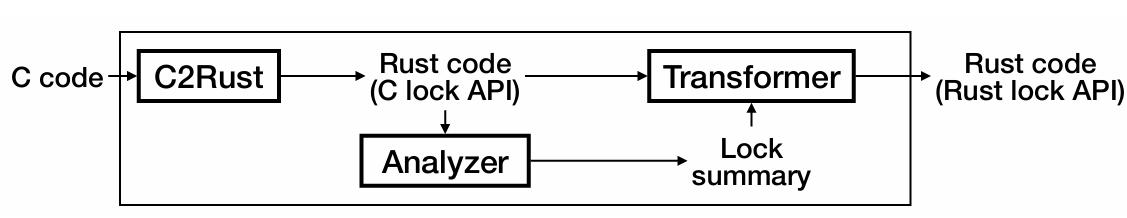
\includegraphics[width=0.8\textwidth]{ch2/assets/concratworkflow.jpg}
\decoRule
\caption[Concrat]{Concrat workflow \parencite{hong2023improving}}
\label{fig:Concrat}
\end{figure}

\break

The tool achieved valid compilable Rust code in 29 of 46 cases collected from the github, 
proving that ownership-based concurrency can be automated even for legacy codebases \parencite{hong2023improving}.
From the 46 cases, 5 of them were also compilable but with a need of a manual fixes. The remain 12 cases were considered failures
classified into three categories:  functions conditionally acquiring locks, function pointers, and pointers to locks \parencite{hong2023improving}.

Concrat focuses on C rather than C++, although its findings are applicable at C++ and also applicable to Boost C++ migration.
Libraries as Boost.Thread and Boost.Asio have a strong dependency on manual synchronization, raw pointers 
and complex ownership patterns. The study has demonstrated that a simple translation of that code to Rust, relying on C2Rust 
or C++ bindings, would preserve the safety risks unless concurrency semantics are explicitly reconstructed.
Concrat's static analysis offers a practical blueprint for the reconstruction providing a lock analysis.

This case study illustrates how automated, semantics-aware transformation can bridge the gap between C++’s flexible 
but unsafe concurrency model and Rust’s strict, verifiable approach, enabling incremental and safer integration 
of Rust into existing C++ ecosystems.

\subsection{“Just Use Rust”: A Best-Case Historical Study of Open Source Vulnerabilities in C}

In this paper the authors provide a historical security analysis of C language projects, based on the most common vulnerabilities
of C and provide answers Rust based for those vulnerabilities. Those vulnerabilities were divide into two groups: the vulnerabilities
Rust could prevent and the vulnerabilities Rust cannot prevent. Within this paper 68 prominent open source projects, as linux 
kernel and Curl, were analyzed in order to map the vulnerabilities. 

The study identified a total of 4,507 vulnerabilities across these projects, 2,257 of which had specific 
Common Weakness Enumeration \gls{CWE} designations. These were mapped to Rust's safety guarantees to determine preventative potential. 
The analysis reveals that a significant majority of historical security issues in C are memory safety errors that 
Rust effectively eliminates at compile time.

\break

\begin{figure}
\centering
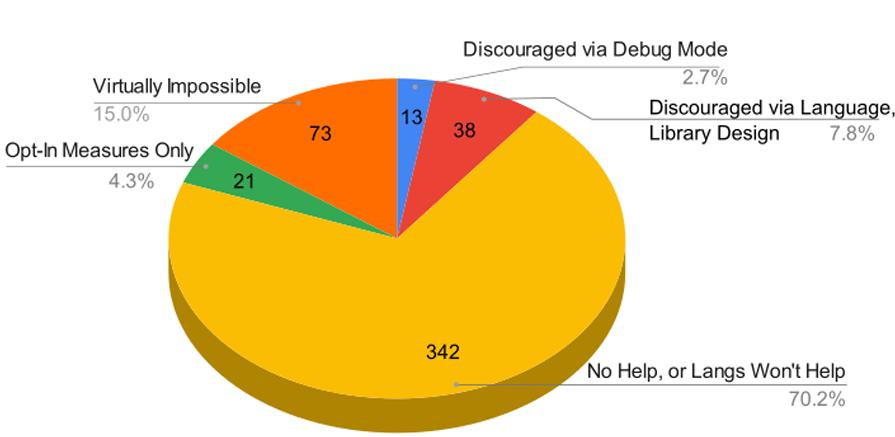
\includegraphics[width=0.8\textwidth]{ch2/assets/rustpreventions.jpg}
\decoRule
\caption[rustpreventions]{Rust Preventions based on \gls{CWE} \parencite{meneely2025just}}
\label{fig:rustpreventions}
\end{figure}

\break

As illustrated in Figure \ref{fig:rustpreventions}, the vulnerabilities are distributed across several categories of potential prevention through Rust. 
Approximately 15.0\% fall into the "Virtually Impossible" category, indicating vulnerabilities that can be prevented by 
Rust's type system and ownership model. In contrast, approximately 70.2\% fall into the "No Help, or Langs Won't Help" category, 
indicating vulnerabilities that cannot be prevented solely through the choice of programming language. 
The remaining vulnerabilities fall into intermediate categories where prevention depends on language features, libraries, 
compiler configurations, or development practices \parencite{meneely2025just}.

Table 1 details the top 20 most common vulnerability types found in the subject projects. 
The data confirms that the two most frequent issues, NULL Pointer Dereference (CWE-476) and Use After Free (CWE-416), 
accounting for nearly 17\% of all analyzed CVEs, are completely preventable in safe Rust \parencite{meneely2025just}.

\break

\begin{table}[h]
\centering
\label{tab:vulnerabilities}
% X column automatically wraps text to fit width
\begin{tabularx}{\textwidth}{|l|X|c|c|l|}
\hline
\textbf{CWE ID} & \textbf{Vulnerability Name} & \textbf{\# CVEs} & \textbf{\# Proj} & \textbf{Rust Prevention} \\ \hline
CWE-476 & NULL Pointer Dereference & 411 & 17 & Virtually Impossible \\ \hline
CWE-416 & Use After Free & 343 & 17 & Virtually Impossible \\ \hline
CWE-125 & Out-of-bounds Read & 145 & 14 & Virtually Impossible \\ \hline
CWE-20 & Improper Input Validation & 105 & 17 & No Help \\ \hline
CWE-190 & Integer Overflow or Wraparound & 100 & 12 & Discouraged (Debug) \\ \hline
CWE-401 & Memory Leak & 96 & 6 & Virtually Impossible \\ \hline
CWE-787 & Out-of-bounds Write & 92 & 15 & Virtually Impossible \\ \hline
CWE-667 & Improper Locking & 86 & 4 & Opt-In Measures \\ \hline
CWE-369 & Divide By Zero & 78 & 4 & Virtually Impossible \\ \hline
CWE-617 & Reachable Assertion & 63 & 6 & Discouraged (Debug) \\ \hline
CWE-362 & Race Condition & 62 & 11 & Discouraged (Design) \\ \hline
CWE-119 & Improper Buffer Restriction & 62 & 14 & Virtually Impossible \\ \hline
CWE-400 & Uncontrolled Resource Consumption & 59 & 15 & No Help \\ \hline
CWE-122 & Heap-based Buffer Overflow & 53 & 12 & Virtually Impossible \\ \hline
CWE-200 & Exposure of Sensitive Information & 45 & 11 & No Help \\ \hline
CWE-120 & Classic Buffer Overflow & 45 & 9 & Virtually Impossible \\ \hline
CWE-908 & Use of Uninitialized Resource & 35 & 5 & Virtually Impossible \\ \hline
CWE-415 & Double Free & 34 & 8 & Virtually Impossible \\ \hline
CWE-770 & Resource Allocation without Limits & 29 & 7 & No Help \\ \hline
CWE-131 & Incorrect Buffer Size Calculation & 26 & 7 & Virtually Impossible \\ \hline
\end{tabularx}
\caption{Top 20 Most Common Vulnerabilities and Rust Prevention Status \parencite{meneely2025just}}
\end{table}

This data suggests that while Rust is not a "silver bullet" for all security issues (such as input validation or logic bugs), 
its adoption could have theoretically prevented the majority of the most severe historical vulnerabilities 
found in these critical infrastructure projects \parencite{meneely2025just}.